\chapter{Background}

\section{Automatic Drum Transcription}

As mentioned, \gls{ADT} describes the task of transcribing symbolic notation for drums from audio. To be even more descriptive, \gls{ADT} can be split into further tasks. From least to most complex we have: \gls{DSC}, where we classify drum instruments from isolated recordings. \gls{DTD}, where we transcribe audio containing exclusively drum instruments. \gls{DTP}, where we transcribe audio containing drum instruments, and additional percussive instruments which the transcription should exclude. Finally, we have \gls{DTM}, which describes the task of drum transcription with audio containing both drum, and melodic instruments.~\cite{8350302}

In this thesis, we will focus on the most complex of these, namely \gls{DTM}. Intuitively, we want to develop a deep learning model which, given input audio, has the ability to detect and classify different drum instrument onsets (events), while selectively ignoring unrelated, melodic instruments.

This task comes with difficulties not seen in the less complex tasks. Zehren et al.~\cite{signals4040042} describes one example, in where \textit{"melodic and percussive instruments can overlap and mask eachother..., or have similar sounds, thus creating confusion between instruments"}.

Deep learning has shown to be a promising method to solve such a task, and several different approaches have been tried, many with great success. Vogl et al.~\cite{vogl2018multiinstrumentdrumtranscription, Vogl2017DrumTV} displayed good results with both a convolutional, and a convolutional-recurrent neural network. Zehren et al.~\cite{signals4040042, zehren2024analyzingreducingsynthetictorealtransfer} focused on datasets, showing that the amount of data and quality of data are equally important to get good performance. Most recently, Chang et al.~\cite{chang2024yourmt3multiinstrumentmusictranscription} explored an autoregressive, language model approach. This approach explored multi-instrument transcriptions, but their results on \gls{ADT} were notable.

This reinforces the fact that there still exist many approaches to attempt, which could lead to a general improvement on \gls{ADT} models.

\section{The Drum Set}

The drum set is a collection of percussive instruments like different drums, cymbals, and possibly different auxillary percussions. A drum set can vary in what it is composed of, however a standard kit usually consists of a snare drum, a bass drum, one or more tom-toms (toms), one or more cymbals (crash and ride), and a hi-hat cymbal~\cite{TheDrumHandbook2003}.

\begin{figure}[H]
    \centering
    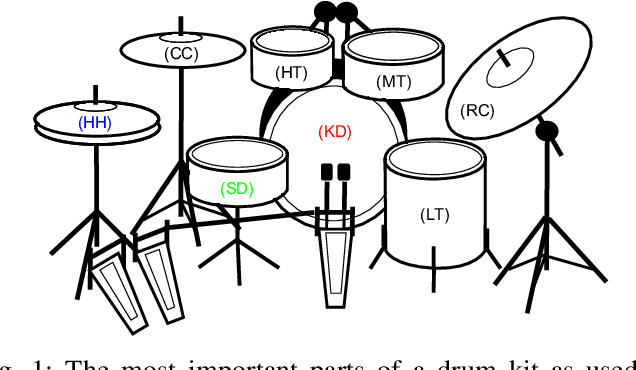
\includegraphics[scale=0.5, trim={0 1cm 0 0},clip]{figures/drumset}
    \caption{Example of the different instruments on the drumset.}
    \label{DrumsetFigure}
\end{figure}

As mentioned, percussion like the drum set, stands in contrast to other musical instruments in that the different ways of playing the same instrument often differ a lot in their \textit{"audible footprint"}. The snare drum, bass drum and hi-hat all have quite different timbres, frequency span, volume, and all in all fundamentally are different instruments.

\begin{figure}[H]
    \centering
    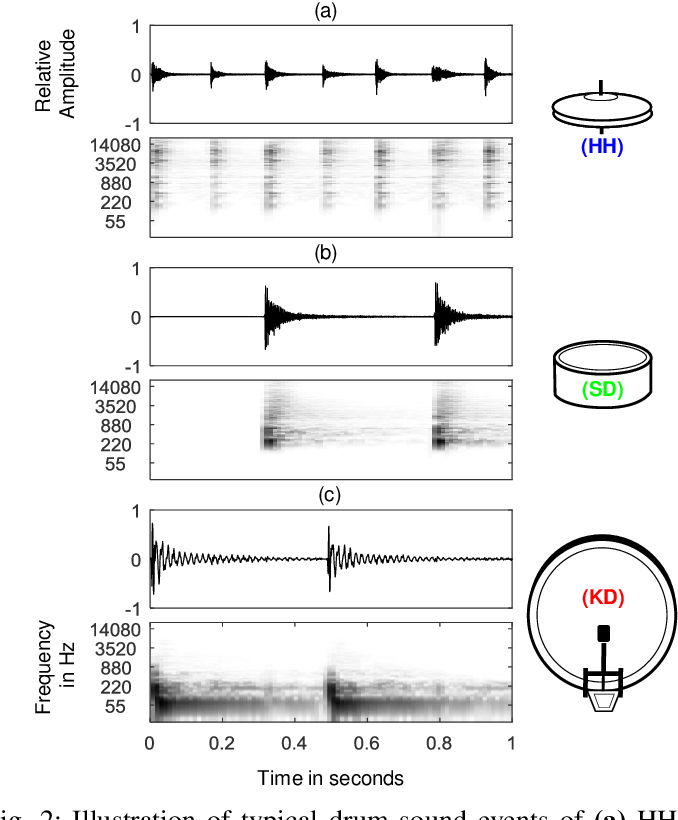
\includegraphics[scale=0.5, trim={0 1cm 0 0},clip]{figures/drumsettimbre}
    \caption{Example of the different audible footprint for drum set percussion.}
    \label{DrumsetTimbreFigure}
\end{figure}

\textcolor{red}{Mention the different drum set instruments. Mention how they all have different musical properties, like frequency, timbre, etc (show waveforms maybe?). Also mention the most fundemental ones, and how Bass, snare and hi-hat are more important than e.g. the mid-tom or something.}

\section{Transcription Task}

\textcolor{red}{\textbf{An introduction to the task, with an image overview over the pipeline (Waveform $\rightarrow$ Spectrogram $\rightarrow$ Neural Network $\rightarrow$ Activation Functions $\rightarrow$ Transcription) should be done here, and is natural to give the reader a thorough understanding of the task before any other information. UNDERSTANDING THE TASK IS THE MOST IMPORTANT PART!}}

\section{Audio}

Sound has be described as \textit{"the sensation caused in the nervous system by vibration of the delicate membranes of the ear."}~\cite{1953fundamentals}. In short, sound is the human perception of acoustic waves in a transition medium, like air. These waves, consisting of vibrating molecules, get sensed by our auditory organs and perceived by the brain. 

Thus sound can be described as the propogation and perception of waves. Mathematically, waves can be studied as signals~\cite{8454362}. To represent these sounds digitally, as \textit{audio}, one can express these waves as a signal, giving rise to the \textit{waveform}. The waveform is a representation of a signal as a graph, and charts the amplitude, or strength of the signal, over time.

\begin{figure}[H]
    \centering
    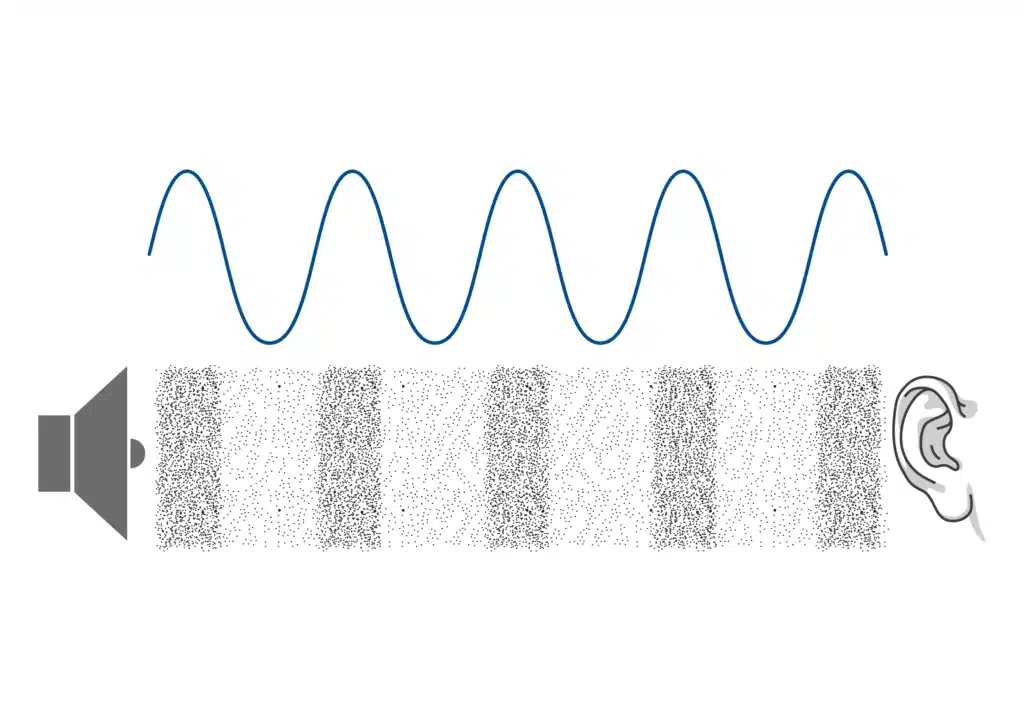
\includegraphics[scale=0.3]{figures/waveform}
    \caption{Soundwave to waveform relationship}
    \label{WaveformFigure}
\end{figure}

For monophonic sound, this waveform is a one-dimensional representation. Even though this is an excellent way of storing audio digitally, it is very compact. There have been deep learning models working directly with these waveforms, e.g. Oord et al.'s WaveNet~\cite{oord2016wavenetgenerativemodelraw}, however the task of parsing and perceiving such a signal is a complex one.

\subsection{Fourier Transform}

The Fourier Transform is a mathematical transformation which, given a frequency, computes its significance, or intensity, in a given signal. As we've established, audio is represented as a signal, and we can therefore use this transform to turn this audio signal into frequency space. 

The fourier transform is a complex transformation. Given a signal $f$, we can compute the integral $$ \widehat{f}(\xi) = \int^{\infty}_{-\infty}{f(x)e^{-i2\pi \xi x} dx} $$ for a frequency $\xi$, resulting in a \textit{complex} number. This number consists of a \textit{real} part and an \textit{imaginary} part. The real part consists of the amplitude of a certain frequency, where as the imaginary part consists of the phase. This information is what allows us to, for a given signal, figure out which frequencies it is made out of and how much each frequency contributes.

By doing such a transform, we turn our temporal data into spectral data. This initively \textit{untangles} our signal into its respective base frequencies. Such an transformation could lessen the complexity of the task, making \textit{understanding} of audio easier.

\begin{figure}[H]
    \centering
    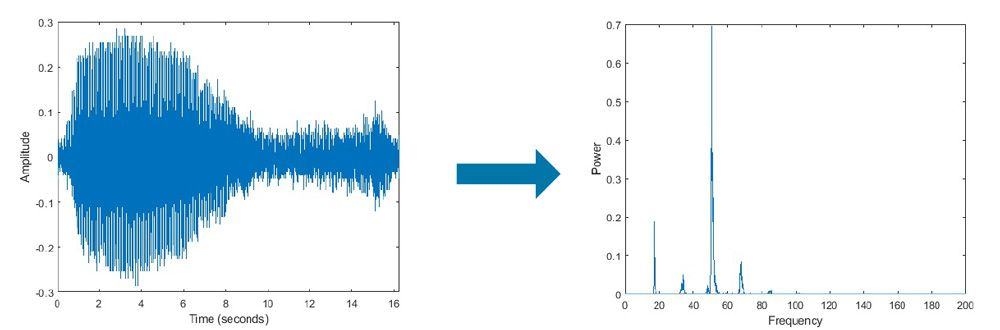
\includegraphics[scale=0.4]{figures/fft.jpg}
    \caption{Application of a Fourier Transform}
    \label{FTFigure}
\end{figure}

Note that the Fourier Transform is invertible, meaning that, given information about each frequency, we can perform a similar integral and reconstruct the original signal. In signal processing, this property is exploited heavily.

\subsection{Discrete Fourier Transform}

The Fourier Transform is defined as an integral over continuous time. On computers, instead of storing signals continuously we store signals using a discrete number of samples. Each signal's \textit{sampling rate} describes how many samples a signal contains per second of audio, and is denoted in \textit{Hz}.

To extract frequency values from these signals, we instead have to use the \gls{DFT}. Intuitively this works as the normal Fourier Transform, but ported to work on discrete-valued signals. It is given by the formula $$ X_k = \sum^{N - 1}_{n=0}{x_n \cdot e^{-i 2\pi \frac{k}{N} n}}, $$ where $k$ denotes the frequency and $N$ the number of discrete samples.

\begin{figure}[H]
    \centering
    %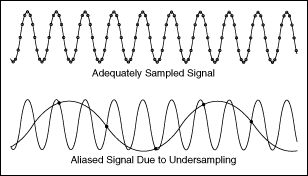
\includegraphics[scale=2.0]{figures/signalaliasing.png}
    \textcolor{red}{Add a example figure of FT vs DFT}
    %\caption{Example of aliasing in an undersampled signal.}
    %\label{AliasingFigure}
\end{figure}

\subsection{Nyquist frequency}

When we discretize a signal, e.g. when going from continuous audio waves in the air to discrete audio signals on a computer, we could lose some information. The discrete representation of the signal is an \textit{approximation} which quality is directly dependent on the sampling rate. The higher the sampling rate, the \textit{closer} we are to the original, continuous signal. However a higher sampling rate comes at the cost of needing to store these signals at a higher precision. A lower sampling rate would need less information stored, but this could also mean a less precise signal approxmation.

\textit{Aliasing} is the phenomena where new frequencies seem to emerge in undersampled signals. For a given discrete signal, the \textit{Nyquist frequency}, equal to half the sampling rate, is the maximum frequency a signal accurately can represent. Thus to prevent aliasing, one would need to store a signal with a sampling rate of at least double the maximum frequency.

\begin{figure}[H]
    \centering
    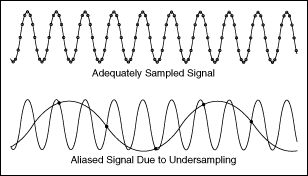
\includegraphics[scale=2.0]{figures/signalaliasing.png}
    \caption{Example of aliasing in an undersampled signal.}
    \label{AliasingFigure}
\end{figure}

Regarding the \gls{DFT}, it here directly follows that the maximum frequency we accurately could extract information about is proportional to the sampling rate of the signal.

\subsection{Fast Fourier Transform}

Keen-eyed computer scientists may have spotted that the \gls{DFT} runs in $\mathcal{O}(n^2)$ time as we, for every frequency in the range $[0, N]$ have to sum over $N$ different values. In other words, the \gls{DFT} algorithm scales quite poorly. Take into account that the standard sampling rate for audio is $44.1 \text{kHz}$, i.e. $44100 \text{Hz}$, then we can see that the \gls{DFT} could be inefficient.~\cite{pras2010sampling}

The \gls{FFT} is an algorithm which solves this problem, and instead computes the \gls{DFT} of a signal within $\mathcal{O}(n\log{n})$ time. Described by Gilbert Strang as \textit{"the most important numerical algorithm of our lifetime"}~\cite{strang1993wavelettransformsversusfourier}, this practically solves our scaling problem, and allows us to efficiently extract spectral information from a signal regardless of sampling rate.

There exist many different implementations of the \gls{FFT}. However the Cooley-Tukey algorithm is by far the most used \gls{FFT} and optimizes calculations through a \textit{divide and conquer} approach, utilizing previous calculations to compute others.~\cite{d3ea2d52-5ab2-3128-8b80-efb85267295d}

\subsection{Short-time Fourier Transform}

The Fourier Transform comes with some drawbacks, notably how by moving from time space into frequency space, we lose temporal information. For certain tasks this might be sufficient, but the temporal dimension is vital when working with transcriptions and \gls{ADT} tasks. We've seen how the Fourier Transform computes the frequencies of a signal, but what happens if we had applied the same transform to smaller, \textit{partitions} of a signal.

This leads us to the \gls{STFT}. By instead of transforming the whole signal, we transform smaller \textit{windows}, we could gain insight into the frequency space while keeping temporal information relatively intact. This turns our data from being one-dimensional into two-dimensional, giving us insight into the intensities of different frequencies, along different timesteps.

\textcolor{red}{Talk more about the partitioning. The window functions applied, and why. Spectral leakage..}

\begin{figure}[H]
    \centering
    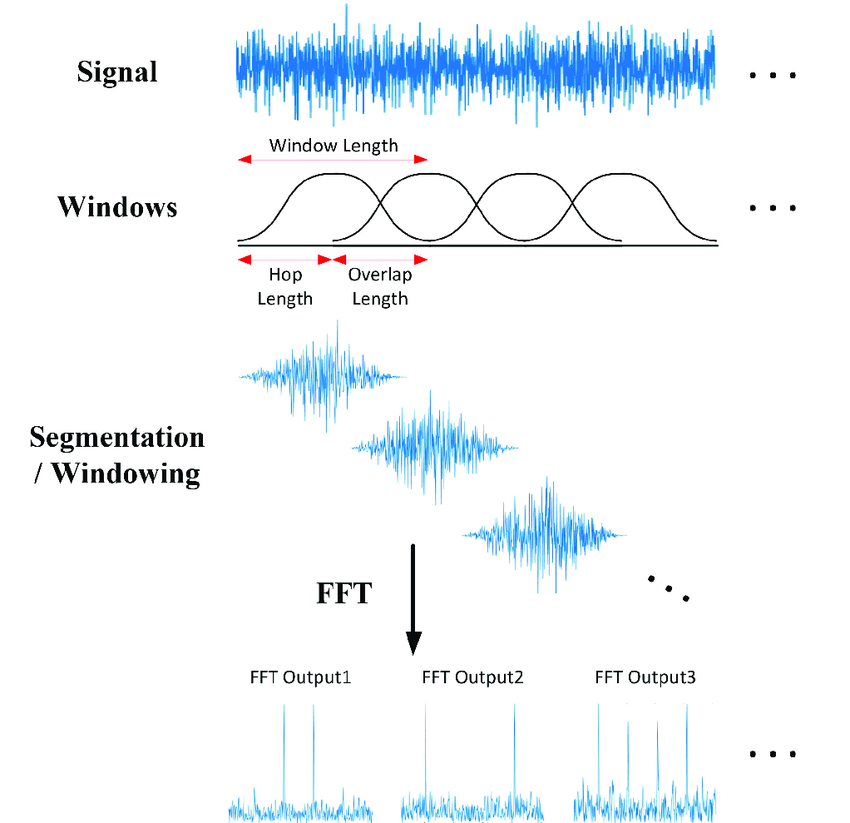
\includegraphics[scale=0.35]{figures/stft}
    \caption{Example of the \gls{STFT}}
    \label{STFTFigure}
\end{figure}

\subsection{Spectrogram}

The \gls{STFT}, as the standard Fourier Transform, returns the data as complex values. To turn these into strictly real values without discarding data, we could compute the spectrogram. This is done by squaring the absolute value of each complex number. 

This results in a 2-dimensional, real representation of our signal. A representation like this is equivalent to an \textit{image}. In this way, we've converted our audible information into visual information. Naturally, these spectrograms can be visualized using e.g. a heatmap.

\begin{figure}[H]
    \centering
    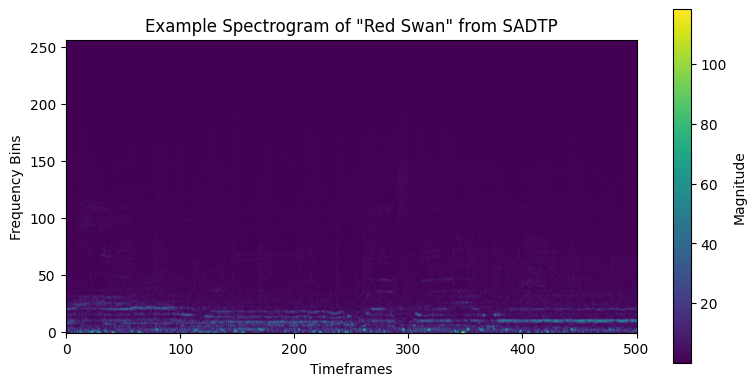
\includegraphics[scale=0.35]{figures/spectrogram}
    \caption{Heatmap of an audio spectrogram.}
    \label{SpectrogramFigure}
\end{figure}

One drawback about the spectrogram is that it contains no information about the phase of the signal it represents. That means it will not be possible to reverse the process and recreate the exact original signal. However, one could try to create an approximation like is done with the Griffin-Lim algorithm~\cite{1164317}.

\subsection{Filters}

Signal frequencies and human perception have a special relationship. We humans percieve logarithmic differences in frequencies as a linear difference in pitch, and we tend to be better at distinguishing differences in lower frequencies than higher. E.g., the notes $\text{A}_2$ and $\text{B}_2$ have the same perceptual pitch difference as $\text{D}_7$ and $\text{E}_7$, even though their difference in frequency, $\text{B}_2 - \text{A}_2 \approx 13.471 \text{Hz}$ and $\text{E}_7 - \text{D}_7 \approx 287.703 \text{Hz}$, are vastly different. As the frequency bins in a spectrogram are linearly spaced, this leads to the spectrogram not representing each frequency equally compared to our perception.

To solve this, we can filter the spectrogram into different bins, more suited to represent our perception of sound. This filtering is done by matrix multiplying our spectrogram with a \textit{filterbank}; a matrix representation of different filters.

\subsubsection{Mel Spectrograms}

The mel scale, presented by Stevens, Volkmann, and Newmann in 1937, is a transformation from the frequency scale to the mel scale. These mels have the property such that a linear difference in mels are percieved as linear differences in pitch. Application of mel-filters result in the \textit{mel spectrogram}, and are widely used when dealing with audio in machine learning, and successful applications have been seen in \gls{AMT}.~\cite{wolfmonheim2024spectralrhythmfeaturesaudio, gardner2022mt3multitaskmultitrackmusic, chang2024yourmt3multiinstrumentmusictranscription, 8350302, gong2021astaudiospectrogramtransformer, zehren2024analyzingreducingsynthetictorealtransfer}

\subsubsection{Logarithmic Filters}

The mel scale was created to mimic human perception of sound, however within \gls{ADT} there is a different trend. By instead using logarithmically spaced filters, centered on the note $\text{A}_4$, we get a \textit{logarithmically filtered spectrogram}. Intuitively one could assume this, instead of mimicing human perception, ports the spectrogram into a format preserving musical relationship and information. This seems to be a standard for \gls{ADT} and has been used extensively by the likes of Vogl et al.~\cite{8350302, vogl2018multiinstrumentdrumtranscription, Vogl2017DrumTV, signals4040042}

\begin{figure}[H]
    \centering
    %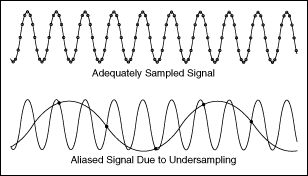
\includegraphics[scale=2.0]{figures/signalaliasing.png}
    \textcolor{red}{Add a example figure of Spectrogram vs Mel vs Logarithmic}
    %\caption{Example of aliasing in an undersampled signal.}
    %\label{AliasingFigure}
\end{figure}

\section{Transcription}

Transcription refers to a process in which we convert information from an audible format, like music, to another medium. This medium then contains a \textit{description} of said audio. As we focus on a musical context, there are a few notable such mediums.

\textcolor{red}{Explain what a transcription is, and what formats they usually are on. Explain what our model is predicting.}

\subsection{Sheet Music}

Sheet music is a written transcription using musical notation that, for a given instrument, contains the \textit{recipe} for a musician to play parts of the original recording. This is the standard when it comes to printing arrangements, and is extensively used by musicians.

Sheet music is typically descriptively exhaustive, and could contain information about musical properties like instrument onsets, tempo, velocity, etc. 

\begin{figure}[H]
    \centering
    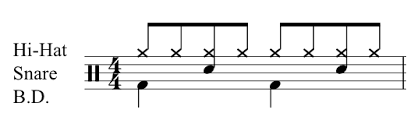
\includegraphics[scale=1.0]{figures/drumsheet}
    \caption{Example sheet music for a drumset}
    \label{DrumsheetFigure}
\end{figure}

\subsection{MIDI Annotations}

\gls{MIDI} is the industry standard for handling music digitally. It is a binary format, containing sequences of commands that allow digital interfaces to \textit{synthesize} music. As it is binary, it is unreadable to us humans without translating it into another format. When computers play \gls{MIDI} arrangements, the \gls{MIDI} sequences are parsed at a constant speed, playing different sounds through \textit{note on}/\textit{note off} events, delayed by time \textit{deltas}. Similar to sheet music, \gls{MIDI} is also very descriptive. And one could say that, intuitively, \gls{MIDI} is to a computer what sheet music is to a musician.

Recently, outputting transcriptions in a \gls{MIDI}-like format has been attempted in \gls{DTM}, and has shown to be promising. Utilizing a sequence-to-sequence \gls{NLP} approach, Garner et al. presented MT3~\cite{gardner2022mt3multitaskmultitrackmusic}, a model inputting spectrograms and outputting \gls{MIDI} events autoregressively. This format was expanded on by Chang et al.'s YourMT3+~\cite{chang2024yourmt3multiinstrumentmusictranscription}, using a \gls{LLM} instead.

\begin{figure}[H]
    \centering
    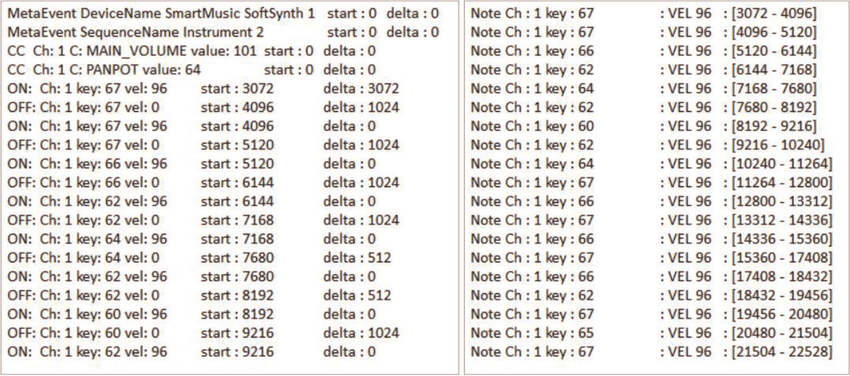
\includegraphics[scale=0.5, trim={0 0 13.8cm 0},clip]{figures/midi}
    \caption{Example MIDI arrangement in a readable format}
    \label{MIDIFigure}
\end{figure}

\textcolor{red}{Accuracy ...}

\subsection{Activation Functions}

In machine learning, the task of detecting instrument onsets could be described as a multi-label sequence labeling task. This involves, for each timeframe in a sequence, predicting a probability, or rather confidence value, that a certain instrument onset happens. In the domain of \gls{MIR} and \gls{AMT}, it has become common place to describe these confidence distributions as \textit{activation functions}; not to be confused with the general deep learning term, activation functions like ReLU or sigmoid.~\cite{Southall2016AutomaticDT, vogl2018multiinstrumentdrumtranscription}

This way of frame-level prediction is extensively used within onset detection in \gls{ADT} and is the approach we will be taking in this thesis.

\begin{figure}[H]
    \centering
    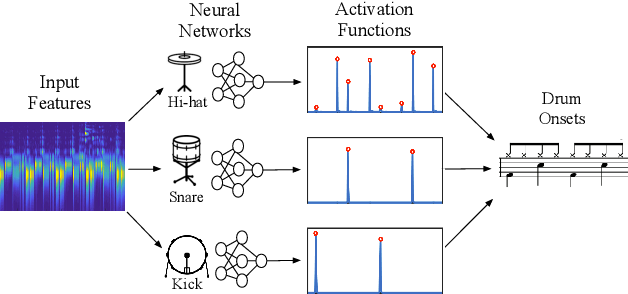
\includegraphics[scale=0.5]{figures/activations.png}
    \caption{Example of \gls{ADT} activation function output}
    \label{ActivationsFigure}
\end{figure}

\subsubsection{Peak-picking}

When predicting activation functions, we need a separate post-processing step to turn these confidence distributions into onset events. By utilizing a standard \textit{peak-picking} algorithm, we can isolate and enhance peaks in these activation functions, and go from a continuous distribution to a collection of discrete events.

The peak-picking algorithm, introduced in its current form by Böck et al.~\cite{Bck2012EvaluatingTO}, defines that a prediction $\hat{y}_n$ at timeframe $n$ is a \textit{peak} if it fulfills the three conditions:
\begin{align*} 
    \hat{y}_n &= \text{max}(\hat{y}_{n - m}, ..., \hat{y}_n, ... \hat{y}_{n + m}), \\ 
    \hat{y}_n &\ge \text{mean}(\hat{y}_{n - a}, ..., \hat{y}_n, ... \hat{y}_{n + a}) + \delta, \\
    n &\ge n_\text{last onset} + w.
\end{align*}

For appropriately trained deep learning models, Vogl et al.~\cite{vogl2018multiinstrumentdrumtranscription} showed that the peak-picking parameters which gave the best results were $m = a = w = 2$ and $\delta = 0.1$.

\section{Performance Measure}

\subsection{Correct Predictions}

Our machine learning models predict instrument onset events on a frame-level basis. In other words, are predictions are very granular, and we need some way to decide when a prediction is correct versus incorrect. In \gls{ADT}, a standard has become to allow a \textit{tolerance window} where event predictions are correct if they lie within a certain time window, often between $25\text{ms}$ and $50\text{ms}$. A side effect of this is that, by shifting our focus to predicted events, we lose information about \textit{not} predicting any events~\cite{inproceedings}.

\subsection{Accuracy}

For classification tasks, a standard performance measure would be \textit{accuracy}: $$ \text{Accuracy} = \frac{\text{TP} + \text{TN}}{\text{TP} + \text{TN} + \text{FP} + \text{FN}}.$$ Summing up correct predictions, \gls{TP} and \gls{TN}, and dividing by total number of predictions, sum of \gls{TP}, \gls{TN}, \gls{FP} and \gls{FN}, we find a model's probability of having a correct prediction.

This performance measure falls short in that it is very susceptible to imbalanced datasets. In \gls{ADT}, most timeframes contain no onset, meaning a naïve predictor would get a high accuracy by never predicting any onsets. Another problem with accuracy is that, due to our tolerance window approach we do not have quantities for \gls{TN}, such that the standard accuracy computation is incomputable.

\subsection{F1-score}

Mentioned above are some of the reasons why \textit{F1-score} has become the typical performance measure within \gls{ADT}. F1-score combines and tries to maximize two different performance measures, namely \textit{precision}; $$ \text{Precision} = \frac{\text{TP}}{\text{TP} + \text{FP}}, $$ and \textit{recall}; $$ \text{Recall} = \frac{\text{TP}}{\text{TP} + \text{FN}}. $$

The precision of a model can tell us how good it is at \textit{hitting} predictions. \textit{Perfect precision} happens when a model has no \gls{FP}, i.e. never predicting an event where one doesn't happen. Recall is similar, but represents the other end of the stick. It tells us how good a model is at \textit{not missing} predictions. \textit{Perfect recall} happens when a model has no \gls{FN}, i.e. never \textit{not} predicting an event where one does happen.

As mentioned, F1-score combines these two measures in an aggregate performance measure by computing their harmonic mean: $$ \text{F1-score} = \frac{2 \cdot \text{Precision} \cdot \text{Recall}}{\text{Precision} + \text{Recall}}. $$ By maximizing F1, we simultaneously maximize both precision and recall as well, reaping all their benefits.

\subsection{Micro vs. Macro}

There are different ways of computing and combining F1-score on multi-label data. Even though they might seem similar, they fundamentally represent different information, and thus the choice in which one to select is crucial.

\textit{Macro F1-score} is computed through the arithmetic mean of the classwise computed F1-scores. Finding a model which maximizes this measure would be similar to finding the model which performes best on each of the separate classes, preventing a class from taking priority due to imbalanced datasets. Relating this to \gls{ADT}, it would mean focusing on transcribing each instrument equally well.

\textit{Micro F1-score} is computed through finding the F1-score with global \gls{TP}, \gls{FP}, \gls{FN} values. Maximizing this would mean prioritizing classes that occur more frequently in the datasets. Such as in \gls{ADT}, this would mean focusing on transcribing instruments which appear often, like the snare or base drum, over rarer instruments like the toms \textcolor{red}{(Somewhere in this master thesis we need a quick introduction to the drums, and which piece of the drumset is which)}. 

For \gls{ADT}, the trend has been to select Micro F1-score as the main performance measure, due to its ability to show a model's \textit{general} performance on musical pieces. We want our model to maximize their ability to transcribe music, not maximize their ability to transcribe each instrument in said music. \gls{ADT}, prioritizing frequent instruments is relevant. As mentioned previously, the more frequent instruments lay the ground work for the fundamentals, and could be said to be more important than scarcely occuring ones.